\section{}
\[
H(s)=\frac{-1000}{(s+1)(s+100)}\,.
\]
\subsection{Bode-Diagramm}
\begin{center}
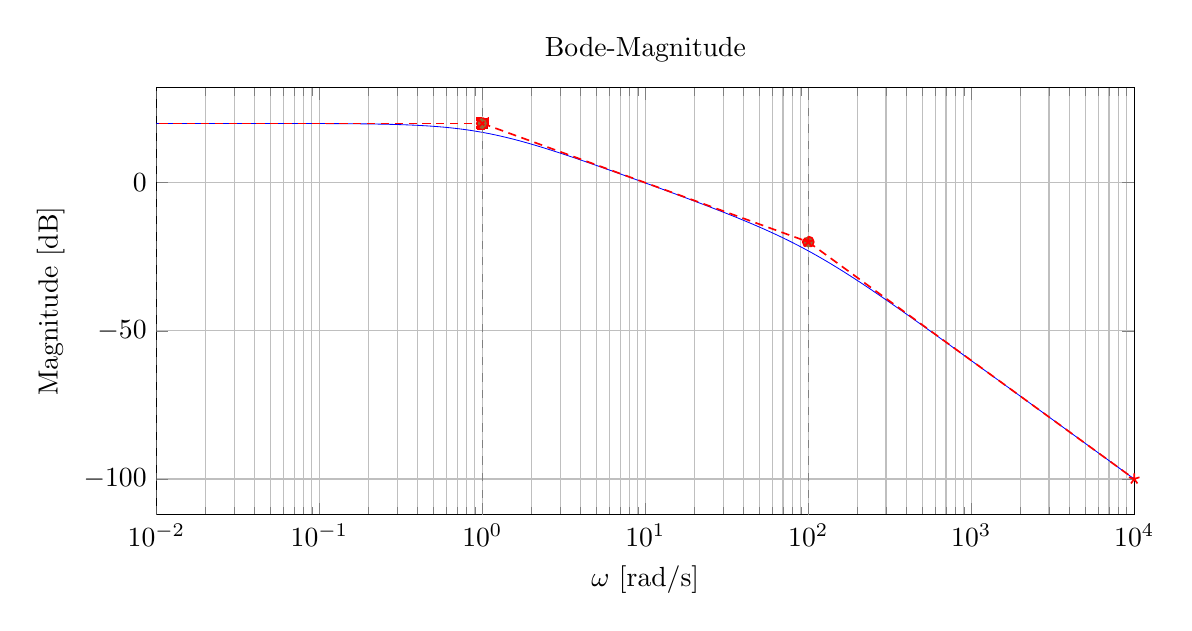
\begin{tikzpicture}
\begin{semilogxaxis}[
  width=14cm,height=7cm,
  xmin=1e-2,xmax=1e4,
  xlabel={$\omega$ [rad/s]},
  ylabel={Magnitude [dB]},
  grid=both,
  title={Bode-Magnitude}
]
\addplot[
  domain=1e-3:1e4,
  samples=800,
  mark=none,
  line width=0.3pt,
  blue
] {60 - 20*ln(sqrt(1 + x^2))/ln(10) - 20*ln(sqrt(10000 + x^2))/ln(10)};
\addplot+[domain=1e-3:1,samples=2,dashed,dash pattern=on 3pt off 2pt,line width=0.6pt,red] {20};
\addplot+[domain=1:1e2,samples=2,dashed,dash pattern=on 3pt off 2pt,line width=0.6pt,red] {20 - 20*ln(x)/ln(10)};
\addplot+[domain=1e2:1e4,samples=2,dashed,dash pattern=on 3pt off 2pt,line width=0.6pt,red] {-20 - 40*ln(x/100)/ln(10)};
\draw[gray,dashed] (rel axis cs:0,0) -- (rel axis cs:0,1);
\draw[gray,dashed] (axis cs:1,\pgfkeysvalueof{/pgfplots/ymin}) -- (axis cs:1,\pgfkeysvalueof{/pgfplots/ymax});
\draw[gray,dashed] (axis cs:100,\pgfkeysvalueof{/pgfplots/ymin}) -- (axis cs:100,\pgfkeysvalueof{/pgfplots/ymax});
\node[gray,anchor=south east] at (axis cs:1,\pgfkeysvalueof{/pgfplots/ymax}) {\scriptsize Pol $\omega_p=1$};
\node[gray,anchor=south east] at (axis cs:100,\pgfkeysvalueof{/pgfplots/ymax}) {\scriptsize Pol $\omega_p=100$};
\end{semilogxaxis}
\end{tikzpicture}
\vspace{6mm}
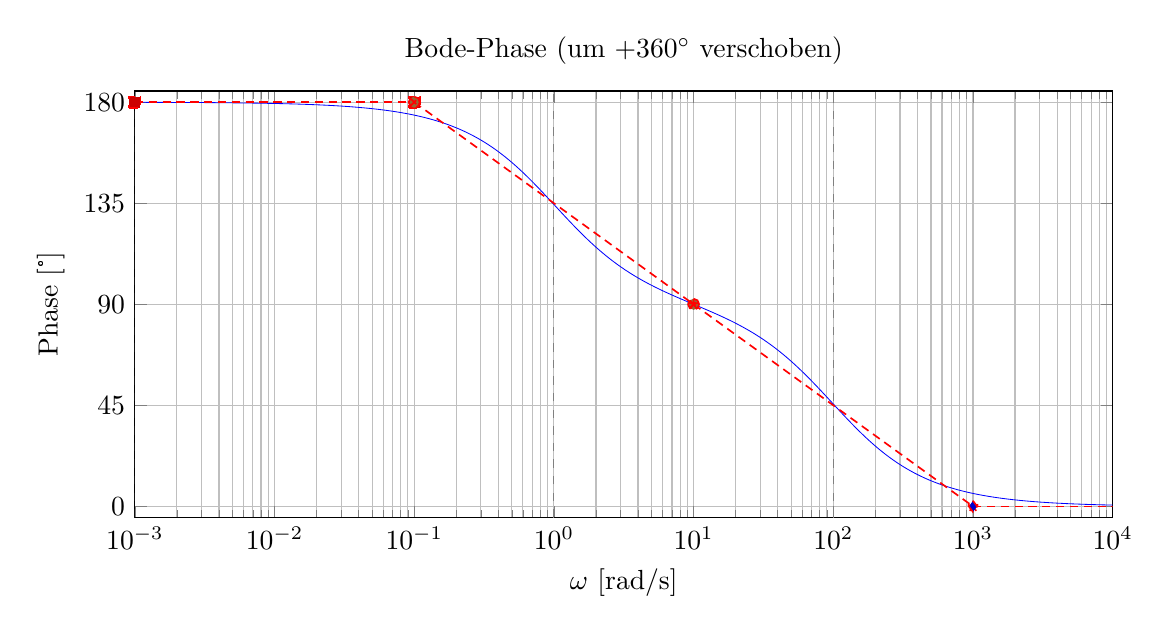
\begin{tikzpicture}
\begin{semilogxaxis}[
  width=14cm,height=7cm,
  xmin=1e-3,xmax=1e4,
  ymin=-5,ymax=185,
  ytick distance=45,
  xlabel={$\omega$ [rad/s]},
  ylabel={Phase [°]},
  grid=both,
  title={Bode-Phase (um $+360^\circ$ verschoben)}
]
\addplot[
  domain=1e-3:1e5,
  samples=800,
  mark=none,
  line width=0.3pt,
  blue
] {180 - atan(x) - atan(x/100)};
\addplot+[domain=1e-3:1e-1,samples=2,dashed,dash pattern=on 3pt off 2pt,line width=0.6pt,red] {180};
\addplot+[domain=1e-1:1e1,samples=2,dashed,dash pattern=on 3pt off 2pt,line width=0.6pt,red] {135 - 45*ln(x)/ln(10)};

\addplot+[domain=1e1:1e3,samples=2,dashed,dash pattern=on 3pt off 2pt,line width=0.6pt,red]{45 - 45*ln(x/100)/ln(10)};
\addplot+[domain=1e3:1e5,samples=2,dashed,dash pattern=on 3pt off 2pt,line width=0.6pt,red]{0};
\draw[gray,dashed] (rel axis cs:0,0) -- (rel axis cs:0,1);
\draw[gray,dashed] (axis cs:1,\pgfkeysvalueof{/pgfplots/ymin}) -- (axis cs:1,\pgfkeysvalueof{/pgfplots/ymax});
\draw[gray,dashed] (axis cs:100,\pgfkeysvalueof{/pgfplots/ymin}) -- (axis cs:100,\pgfkeysvalueof{/pgfplots/ymax});
\node[gray,anchor=south east] at (axis cs:1,\pgfkeysvalueof{/pgfplots/ymax}) {\scriptsize Pol $\omega_p=1$};
\node[gray,anchor=south east] at (axis cs:100,\pgfkeysvalueof{/pgfplots/ymax}) {\scriptsize Pol $\omega_p=100$};
\end{semilogxaxis}
\end{tikzpicture}
\end{center}
\newpage
\subsection{Erklärung}
\vspace{5mm}
\begin{description}[leftmargin=1.2em,labelsep=.6em,font=\bfseries]
\item[Schritt 1] Konstante und Normierung: 
\(H(s)=\dfrac{-1000}{(s+1)(s+100)}=-10\,\dfrac{1}{(1+s)(1+s/100)}\).
DC-Wert \(H(0)=-10\Rightarrow |H|_{\mathrm{DC}}=20\,\mathrm{dB}\). Das negative Vorzeichen bewirkt eine konstante Zusatzphase; hier wird die Phase um \(+360^\circ\) angehoben, sodass sie von \(180^\circ\) (für \(\omega\ll1\)) nach \(0^\circ\) (für \(\omega\gg100\)) verläuft.
\item[Schritt 2] Pol bei \(\omega_{p1}=1\,\mathrm{rad/s}\): ab \(\omega=1\) sinkt die Magnitude mit \(-20\,\mathrm{dB/dec}\). Exakt: Zusatzdämpfung \(-10\log_{10}2\approx-3.01\,\mathrm{dB}\). Phasenanteil (verschoben): Geradennäherung \(135^\circ-45^\circ\log_{10}\omega\) über \([0.1,10]\).
\item[Schritt 3] Pol bei \(\omega_{p2}=100\,\mathrm{rad/s}\): ab \(\omega=100\) weitere Steigungsänderung \(-20\,\mathrm{dB/dec}\)\(\Rightarrow\) Gesamtslope \(-40\,\mathrm{dB/dec}\) für \(\omega\gg100\). Phasenanteil (verschoben): \(45^\circ-45^\circ\log_{10}(\omega/100)\) über \([10,10^5]\). Grenzwerte: \(|H(\j\omega)|_{\mathrm{dB}}\sim -40\log_{10}(\omega/100)-20\) für \(\omega\to10^5\); \(\angle H(\j\omega)\to 0^\circ\).
\end{description}

\vspace{0.5cm}
\medskip
\noindent\textbf{Stückweise Näherung}
\[
|H(\j\omega)|_{\mathrm{dB}}\approx
\begin{cases}
20,& \omega\ll1,\\[4pt]
20-10\log_{10}2,& \omega=1,\\[4pt]
20-20\log_{10}\omega,& 1\ll\omega\ll100,\\[4pt]
-20-10\log_{10}2,& \omega=100,\\[4pt]
-20-40\log_{10}(\omega/100),& \omega\gg100,
\end{cases}
\qquad
\]
\newpage